\documentclass[modern]{aastex63}

\usepackage{amsmath}

\newcommand{\dd}{\ensuremath{\mathrm{d}}}
\newcommand{\diff}[2]{\frac{\dd #1}{\dd #2}}

% Affiliations
\newcommand{\flatironCCA}{Center for Computational Astrophysics, Flatiron Institute, 162 5th Ave, New York NY 10010, United States}
\newcommand{\stonybrook}{Department of Physics and Astronomy, Stony Brook University, Stony Brook NY 11794, United States}

\begin{document}

\title{Re-Weighting Existing Samples to a Population Analysis}
\author{Will M. Farr}
\email{will.farr@stonybrook.edu}
\email{wfarr@flatironinstitute.org}
\affiliation{\stonybrook}
\affiliation{\flatironCCA}

\author{Thomas A. Callister}
\email{thomas.callister@flatironinstitute.org}
\affiliation{\flatironCCA}

\begin{abstract} We show how to re-weight pre-existing parameter samples to
obtain samples distributed according to a hierarchical population analysis.  We
discuss the behavior of the marginalized distribution for single-event
parameters in a hierarchical population analysis. \end{abstract}

\section*{ }

For an alternative presentation of essentially identical material, see
\citet{Hogg2010}.

It is a common problem in astronomy to have a collection of observations of some
objects from a population in need of a simultaneous analysis of the population
properties and object properties.  Such analyses are called ``hierarchical''
because they naturally separate into several distinct ``levels.''  To be a bit
more mathematically precise: we are presented with a set of data,
%
\begin{equation}
  D \equiv \left\{ d_i \mid i = 1, \ldots, N \right\},
\end{equation}
%
consisting of $N$ distinct data sets, $d_i$, each representing some measurement
of an object.  Each object may have parameters, $\theta_i$, that are of
interest.  We think that the set of parameters,
%
\begin{equation}
  \Theta \equiv \left\{ \theta_i \mid i = 1, \ldots, N \right\},
\end{equation}
%
comes to us as fair draws\footnote{If the draws are not fair, then the sample is
said to suffer from \emph{selection effects}; in this case see
\citet{Loredo2004,Messenger2013,Mandel2019}.  \citet{Loredo2004,Mandel2019} also
describe how to fit a \emph{rate} of objects from such observations.} from a
population distribution, which may in turn depend on some paramteters,
$\lambda$:
%
\begin{equation}
  \theta_i \sim p\left( \theta \mid \lambda \right).
\end{equation}
%
We assume that we know enough about the data generating, or measurement, process
that we can write down a probabilistic description of the data conditioned on
the parameters $\theta$; this function is commonly called the ``likelihood:''
%
\begin{equation}
  d_i \sim p\left( d \mid \theta_i \right).
\end{equation}
%
(Note that $\theta_i$ can contain both parameters that are \emph{intrinsic} to
the object, and also parameters that describe the measurement process for that
object---detector noise levels, or calibration parameters, for example---and
that the population distribution can be both an \emph{intrinsic} population and
also a model of the \emph{distribution} of such measurement parameters.)  A
graphical description of our hierarchical model appears in Figure \ref{fig:pgm}.

\begin{figure}
  \begin{center}
  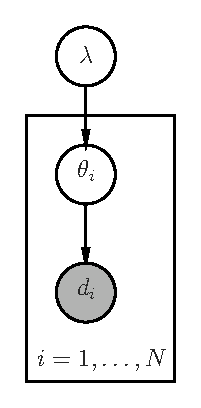
\includegraphics[height=0.5\columnwidth]{pgm}
\end{center}
%
  \caption{\label{fig:pgm} A graphical description of our hierarchical model.
  Each node in the graph is a variable.  Shaded nodes are \emph{observed}
  variables whose values are conditioned on in the analysis.  An arrow
  connecting two nodes represents a distribution of the target node conditioned
  on the source node's value.}
%
\end{figure}

If all these distributions are available to us, then it is straightforward to
sample over the joint distribution of $\Theta$ and $\lambda$ given the data $D$.
Impose a prior on $\lambda$, $p\left( \lambda \right)$; then\footnote{We are
here implicitly assuming that the data generating process is such that
\emph{once conditioned on parameters $\theta$} successive observations are
independent of each other.  This is almost certainly false, but may be ``true
enough'' for our purposes, particularly if there are parameters describing
systematic or ``calibration'' effects in our instrument in each $\theta_i$.}
%
\begin{equation}
  \label{eq:joint-posterior}
  p\left( \Theta, \lambda \mid D \right) \propto \left[ \prod_{i=1}^N p\left( d_i \mid \theta_i \right) p\left( \theta_i \mid \lambda \right) \right] p\left( \lambda \right),
\end{equation}
%
and your favorite stochastic sampling method\texttrademark{} can be used to draw
samples in the (possibly high-dimensional) space of $\Theta$ and $\lambda$.
However, the more common situation is that we are provided instead with a
\emph{catalog} of objects and parameters already inferred from them according
to some prior.  Thus, we have a set of $M$ samples,
%
\begin{equation}
  \left\{ \theta_i^{(j)} \mid j = 1, \ldots, M \right\},
\end{equation}
%
where each sample is drawn from a posterior with a prior $p_0$:
%
\begin{equation}
  \theta_i^{(j)} \sim p\left( d_i \mid \theta \right) p_0\left(\theta \right).
\end{equation}

A common trick in this situation \citep{Hogg2010} is to give up on sampling in
$\Theta$, and integrate the $\theta_i$ out of Eq. \eqref{eq:joint-posterior}:
%
\begin{equation}
  p\left( \lambda \mid D \right) \propto \left[ \prod_{i=1}^N \int \dd \theta_i p\left( d_i \mid \theta_i \right) p\left( \theta_i \mid \lambda \right) \right] p\left( \lambda \right) \equiv p\left( D \mid \lambda \right) p\left( \lambda \right).
\end{equation}
%
The integrals inside the product can be approximated (up to ignorable constants)
using importance sampling with the samples from our catalog, $\theta_i^{(j)}$:
%
\begin{equation}
  \label{eq:marginal-population}
  p\left( \lambda \mid D \right) \propto \left[ \prod_{i=1}^N \left\langle \frac{p\left(\theta \mid \lambda \right)}{p_0\left( \theta \right)} \right\rangle_{\theta_i^{(j)}} \right] p\left( \lambda \right),
\end{equation}
%
where the average is taken over the samples $\theta_i^{(j)}$.  Here the ratio of
the population distribution to the catalog prior is the \emph{importance weight}
for each of the $\theta_i^{(j)}$.  Depending on the number of samples associated
to each object in the catalog and the relative widths of the likelihood, catalog
prior, and population, this procedure can go awry; but often it is good enough,
and its simplicity combined with the (often dramatic) reduction in
dimensionality (the components of $\Theta$ often dominate the number of degrees
of freedom in $\lambda$) argues for using it when possible.

Sometimes we are only interested in the population parameters, $\lambda$; in
this case the individual-object parameters $\Theta$ are a nuisance anyway, and
we need not worry about integrating them out.  However, we are often interested
in \emph{both} the population and individual-level parameters; and sometimes we
are only using the population to improve estimates of individual-level
parameters by (partially) pooling information across observations
\citep{Lieu2017}.  In this case we must recover samples of $\Theta$ after we
have samples from the marginal distribution over population parameters.

Recall that it is a theorem of probability that
%
\begin{equation}
  \label{eq:joint-conditional-relation}
  p\left( \Theta, \lambda \mid D \right) = p\left( \Theta \mid \lambda, D \right) p\left( \lambda \mid D \right).
\end{equation}
If we are given samples, $\lambda^{(k)}$, drawn from $p\left( \lambda \mid D \right)$,
%
\begin{equation}
  \lambda^{(k)} \sim p\left( \lambda \mid D \right),
\end{equation}
%
then augmenting each $\lambda^{(k)}$ with a set $\Theta^{(k)}$, where each $\theta_i^{(k)}$
is drawn from
%
\begin{equation}
  \label{eq:conditional-theta}
  \theta_i^{(k)} \sim p\left( d_i \mid \theta \right) p\left( \theta \mid \lambda^{(k)} \right),
\end{equation}
%
will produce a draw from the joint distribution over $\Theta$ and $\lambda$.
This works because
%
\begin{equation}
  p\left( d_i \mid \theta \right) p\left( \theta \mid \lambda^{(k)} \right) \propto p\left( \theta \mid \lambda, D \right),
\end{equation}
%
with the constant of proportionality \emph{independent} of $\Theta$ at fixed $D$
and $\lambda$.  A draw from Eq.\ \eqref{eq:conditional-theta} can be
accomplished by choosing randomly one of the existing catalog samples
$\theta_i^{(j)}$ with weight, $w_i^{(j)}$, proportional to \citep{Hogg2010}
%
\begin{equation}
  \label{eq:population-weights}
  w_i^{(j)} \propto \frac{p\left( \theta_i^{(j)} \mid \lambda^{(k)} \right)}{p_0 \left( \theta_i^{(j)} \right)}.
\end{equation}

So, to summarize, here is the algorithm for sampling from the joint distribution
of $\Theta$ and $\lambda$ given $D$ and a catalog of samples, $\theta_i^{(j)}$
drawn from a catalog posterior with prior $p_0\left(\theta\right)$.
\begin{enumerate}
%
  \item Use a stochastic sampler to draw samples $\lambda^{(k)}$ from Eq.\ \eqref{eq:marginal-population}.
%
  \item For each sample, $\lambda_k$, and each object $i$, draw a random catalog
  sample, $\theta_i^{(k)}$ from the $\theta_i^{(j)}$ with weights given by Eq.\
  \eqref{eq:population-weights}.
%
\end{enumerate}

The pairs of $\lambda^{(k)}$, and the associated set of catalog draws,
$\Theta^{(k)}$, constitute a sample from the joint distribution on $\Theta$ and
$\lambda$ defined in Eq.\ \eqref{eq:joint-posterior}, and can be used to
estimate population properties, individual-event properties informed by a
population, correlations between population properties and individual-event
properties, etc.

In the case where we are not interested in samples $\lambda$ at all, we can also
integrate out $\lambda$ in Eq.\ \eqref{eq:joint-conditional-relation}.  We will
need the properly-normalized version of Eq.\ \eqref{eq:conditional-theta} since
the normalization depends on $\lambda$:
%
\begin{equation}
  p\left( \theta_i \mid \lambda, D \right) = \frac{p\left( d_i \mid \theta_i \right) p\left( \theta_i \mid \lambda\right)}{p\left( d_i \mid \lambda \right)} = \frac{p\left( d_i \mid \theta_i \right) p\left( \theta_i \mid \lambda\right)}{\int \dd \theta \, p\left( d_i \mid \theta\right) p\left( \theta \mid \lambda \right)}.
\end{equation}
%
Then the marginal distribution for $\theta_i$ is
%
\begin{equation}
  \label{eq:theta-marginal}
  p\left( \theta_i \mid D \right) \propto p\left( d_i \mid \theta_i \right) \int \dd \lambda \, \frac{1}{p\left( d_i \mid \lambda \right)} p\left( \theta_i \mid \lambda \right) p\left( \lambda \mid D \right).
\end{equation}
%
Note that the evidence for object $i$ modifies what otherwise would be the
posterior expectation over $\lambda$ of the population distribution for
$\theta_i$.   Assuming, again, that we have posterior samples $\theta_i^{(k)}$
drawn from a catalog with prior $p_0\left(\theta \right)$ and posterior samples
for $\lambda$ drawn from the marginal posterior, $\lambda^{(l)} \sim p\left(
\lambda \mid D \right)$, this can be approximated as
%
\begin{equation}
  \label{eq:theta-marginal-samples}
  p\left( \theta_i \mid D \right) \propto p\left( d_i \mid \theta_i \right) \left\langle p\left( \theta_i \mid \lambda^{(l)} \right) \left[\left\langle \frac{p\left( \theta_i^{(k)} \mid \lambda^{(l)} \right)}{p_0 \left( \theta_i^{(k)} \right)} \right\rangle_{\theta_i^{(k)}} \right]^{-1} \right\rangle_{\lambda^{(l)}},
\end{equation}
%
or, expressed as importance weights for resampling the $\theta^{(k)}_i$
%
\begin{equation}
  \label{eq:theta-marginal-weights}
  w_i^{(k)} \propto \frac{1}{p_0\left( \theta_i^{(k)} \right)} \left\langle p\left( \theta_i^{(k)} \mid \lambda^{(l)} \right) \left[\left\langle \frac{p\left( \theta_i^{(k')} \mid \lambda^{(l)} \right)}{p_0 \left( \theta_i^{(k')} \right)} \right\rangle_{\theta_i^{(k')}} \right]^{-1} \right\rangle_{\lambda^{(l)}},
\end{equation}
%
where we have introduced the index $k'$ to the inner expectation value to
emphasize that it should be taken independently of the outer expectation over
samples of $\theta_i$. This expression is equivalent to Eq.\ (6) of
\citet{Callister2019}.

Eq.\ \eqref{eq:theta-marginal} and its implementation in Eqs.\
\eqref{eq:theta-marginal-samples} and \eqref{eq:theta-marginal-weights} are
equivalent to imposing a prior on $\theta_i$ that comes from the population
distribution weighted by the ``leave one out'' posterior on
$\lambda$:\footnote{It seems like this must be a well-known fact---probably it
appears in \citet{Gelman2013}---but I am not familiar with it.}
%
\begin{equation}
  p\left( \theta_i \mid D \right) \propto p\left( d_i \mid \theta_i \right) \int \dd \lambda \, p\left( \theta_i \mid \lambda \right) p\left( \lambda \mid D \backslash d_i \right).
\end{equation}
%

\clearpage

\bibliography{reweighting}

\end{document}
